\section{Data Processing}

Before concluding anything from the data, it is first analysed to check if the made assumptions are valid. The assumptions include a stationary channel, uncorrelated samples and finally that the data is Rayleigh distributed.

\subsection{Raw data}

In total 4.184.460 samples have been collected, the values are represented in \autoref{fig:rawFadingMeas}. Here all the space samples has been concatenated to visualize the data.

\begin{figure}[H]
\centering
\includegraphics[height = \textwidth, angle = -90]{figures/rawFadingMeas.pdf}
\caption{The measured samples spaced in frequency and space.}
\label{fig:rawFadingMeas}
\end{figure}


\subsection{Stationarity}
To see if the channel is stationary is to check if the measurements conform to the criteria of \gls{WSSUS}. This is done by checking \gls{WSS} in the frequency domain} and \gls{US} in the spatial domain. The criteria for this is a constant mean and a autocorrelation that is only dependent on delay between samples \citep[ch. 5]{The_Mobile_Radio_Propagation_Channelbook}. 

\textbf{Frequency domain mean}

The data is structured in 3 domains freq x antenna x walk/space, with N, M and K being the number of points in each dimension. To analyse stationarity in frequency an average is taken across the other two domains as:

\begin{equation}\label{eq:freqMean}
freqData_{(n)} = \frac{1}{K\cdot M}\sum_{k = 1}^{K}\sum_{m = 1}^{M} data_{(n,m,k)}
\end{equation}

\begin{figure}[H]
\centering
%\includegraphics[height = \textwidth, angle = -90]{figures/meanFading.pdf}
% This file was created by matlab2tikz.
%
%The latest updates can be retrieved from
%  http://www.mathworks.com/matlabcentral/fileexchange/22022-matlab2tikz-matlab2tikz
%where you can also make suggestions and rate matlab2tikz.
%
\definecolor{mycolor1}{rgb}{0.00000,0.44700,0.74100}%
%
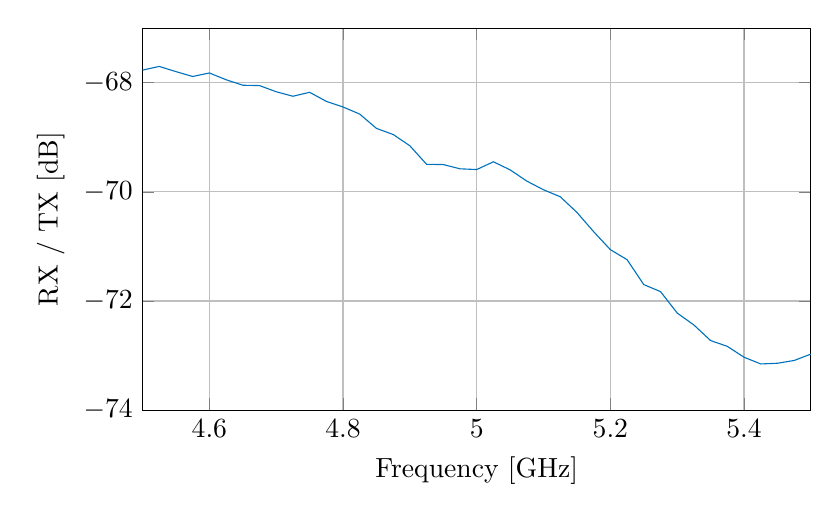
\begin{tikzpicture}

\begin{axis}[%
width=0.7\textwidth,
height=0.4\textwidth,
at={(0.758in,0.481in)},
scale only axis,
xmin=4.5,
xmax=5.5,
xlabel={Frequency [GHz]},
xmajorgrids,
ymin=-74,
ymax=-67,
ylabel={RX / TX [dB]},
ymajorgrids,
axis background/.style={fill=white}
]
\addplot [color=mycolor1,solid,forget plot]
  table[row sep=crcr]{%
4.5	-67.7676892980713\\
4.525	-67.7004021954752\\
4.55	-67.7955301958539\\
4.575	-67.8845412993962\\
4.6	-67.8205218880063\\
4.625	-67.9439627079413\\
4.65	-68.04512612016\\
4.675	-68.051565781706\\
4.7	-68.1644910960917\\
4.725	-68.2469599638715\\
4.75	-68.1744447064323\\
4.775	-68.3408515759533\\
4.8	-68.4431912057773\\
4.825	-68.5744291919179\\
4.85	-68.8363636692087\\
4.875	-68.9480881021396\\
4.9	-69.1549059751271\\
4.925	-69.4947511904151\\
4.95	-69.4993310363175\\
4.975	-69.5769572316811\\
5	-69.5906628312393\\
5.025	-69.4483437709345\\
5.05	-69.5961078771687\\
5.075	-69.8026690275714\\
5.1	-69.9616513128938\\
5.125	-70.0889574328478\\
5.15	-70.3770813009446\\
5.175	-70.7298661505624\\
5.2	-71.0591359058608\\
5.225	-71.2429090613138\\
5.25	-71.6994261918864\\
5.275	-71.8280447931612\\
5.3	-72.2209086728416\\
5.325	-72.4401711956896\\
5.35	-72.7258613771483\\
5.375	-72.8313187431047\\
5.4	-73.0312002594864\\
5.425	-73.154105653938\\
5.45	-73.1413033949649\\
5.475	-73.0904973481192\\
5.5	-72.9729692416908\\
};
\end{axis}
\end{tikzpicture}%
\caption{Average values across the frequency as per \autoref{eq:freqMean}, with values converted from linear scale to dB.}
\label{fig:meanFading}
\end{figure}

It can be seen that there is a drop of around 4 dB across the frequency, this drop can be explained by 2 factors first the antenna gain varies with around 2 dB across the frequency span \appref{ant_adix}, the other part is the \gls{PL} is dependent on frequency, by comparing PL of a free space path loss model, it can be seen that there is a drop of 1.75 dB going from 4.5 GHz to 5.5 GHz. Those two factors together can explain the drop in mean power across the span. As this can be explained the data is adjusted as:

\begin{equation}
data2_{(:,:,k)} =  data_{(:,:,k)} \oslash \left(freqData\cdot ones(1,M)\right), \quad k = (1,2,...,K)
\end{equation}

\textbf{Spatial domain mean}

Likewise as the frequency domain the average is taken across the other domains, here it is assumed that the antennas even though spaced is a separate and stationary domain due to their closeness. The average is found based on the frequency corrected data as:

\begin{equation}\label{eq:spaceMean}
spaceData_{(k)} = \frac{1}{N\cdot M}\sum_{n = 1}^{N}\sum_{m = 1}^{M} data2_{(n,m,k)}
\end{equation}

To visualize the data is restructured such that it matches the area it has been taken in see \autoref{Environment}. The data was collected by walking forth and back in the room with approx. 42 sweeps per meter or 210 sweeps per stretch. As every second stretch was walking back it has to be reversed to visualize the samples side by side. 



\begin{figure}[H]
\captionsetup{belowskip=0em}
\centering
\begin{subfigure}[b]{0.29\textwidth}
\includegraphics[width=\textwidth]{figures/Not_Norm_space_1.png}
\caption{Low height \\ approx. 70 cm}
\label{Not_norm_low}
\end{subfigure}
\begin{subfigure}[b]{0.29\textwidth}
\includegraphics[width=\textwidth]{figures/Not_Norm_space_2.png}
\caption{Medium height \\ approx. 120 cm}
\label{Not_norm_medium}
\end{subfigure}
\begin{subfigure}[b]{0.29\textwidth}
\includegraphics[width=\textwidth]{figures/Not_Norm_space_3.png}
\caption{High height \\ approx. 170 cm}
\label{Not_norm_high}
\end{subfigure}
\begin{subfigure}[b]{0.1\textwidth}
\includegraphics[width=\textwidth]{figures/Not_Norm_space_colorbar.png}
\end{subfigure}
\captionsetup{belowskip=-1.5em}
\caption{The measurements is restructured to be approximately where they was measured compared to each other.}
\label{fig:Not_norm_space}
\end{figure}

It can be seen from \autoref{fig:Not_norm_space} that the power level in the middle of the room is stronger than on the borders. The reason for this is believed to be the directionality of the transmit antenna. The transmit antenna was located outside and shooting in to the room as can be seen on \autoref{antennadoor}, so the main lobe might have been reflected from the wall directly to the middle of the measurement area. Because of this the area can not be said to be stationary so to combat this a moving average is used to normalize the mean power level across the area. The drawback of using a moving average is that it might affect the fading in the measurement, therefore as many point as possible should be in the average to make the influence as little as possible, however if too many points is in the average the stationarity issue would not be solved. It is chosen to average across 41 space samples.

\begin{align}
&MA = \frac{1}{41}\cdot \Big(spaceData*ones(41,1)\Big) \\
data3_{(:,:,k)} = data2_{(:,:,k)} &\oslash \left(MA_{\left(\frac{41-1}{2}:N+\frac{41-1}{2}\right)}\cdot ones(1,M)\right), \quad k = (1,2,...,K)
\end{align}

The result of the normalization can be seen on \autoref{fig:Norm_space}.

\begin{figure}[H]
\captionsetup{belowskip=0em}
\centering
\begin{subfigure}[b]{0.29\textwidth}
\includegraphics[width=\textwidth]{figures/Norm_space_1.png}
\caption{Low height \\ approx. 70 cm}
\label{Norm_low}
\end{subfigure}
\begin{subfigure}[b]{0.29\textwidth}
\includegraphics[width=\textwidth]{figures/Norm_space_2.png}
\caption{Medium height \\ approx. 120 cm}
\label{Norm_medium}
\end{subfigure}
\begin{subfigure}[b]{0.29\textwidth}
\includegraphics[width=\textwidth]{figures/Norm_space_3.png}
\caption{High height \\ approx. 170 cm}
\label{Norm_high}
\end{subfigure}
\begin{subfigure}[b]{0.1\textwidth}
\includegraphics[width=\textwidth]{figures/Norm_space_colorbar.png}
\end{subfigure}
\captionsetup{belowskip=-1.5em}
\caption{The normalize measurements is restructured to be approximately where they was measured compared to each other.}
\label{fig:Norm_space}
\end{figure}

It can be concluded based on this that the mean was not constant during the measurement, however due to the normalization the mean of \textit{spaceData2} can be considered to be constant across all measurements. The last check to see if the channel is \gls{WSS} is to check if the autocovariance function is only dependent on sample shift, this is also done in both the frequency domain and spatial domain.

\textbf{Frequency domain correlation}

It needs to be checked if:
\begin{equation}\label{eq:autocovariance_check}
R(n,n+\Delta n) = R(\Delta n) 
\end{equation}

First the the sample mean and sample variance is found for each point in space as:

\begin{align}
\mu_{(m,k)} &= \frac{1}{N}\sum_{n = 1}^{N} data3_{(n,m,k)} \\
s_{f,(m,k)}^2 &= \frac{1}{N-1}\sum_{n = 1}^{N} \left( data3_{(n,m,k)} - \mu_{(m,k)} \right)^2 
\end{align}

Each element in space the cross covariance matrix is found as the sample covariance divided with the sample variance:
\begin{equation}
C(n,n+\Delta n,m,k) = \frac{\left(data3_{(n,m,k)}-\mu_{(m,k)}\right)\cdot \left(data3_{(n+\Delta n,m,k)}-\mu_{(m,k)}\right)}{s_{f,(m,k)}^2}
\end{equation}

The average across all space samples are then found as:
\begin{equation}
R(n,n+\Delta n) = \frac{1}{K\cdot M}\sum_{k = 1}^{K}\sum_{m = 1}^{M} C(n,n+\Delta n,m,k)
\end{equation}


The final step is to show that \autoref{eq:autocovariance_check} is true. If this is true all diagonal lines in R would have a constant value, that implies that the variance across the diagonal line elements is 0. 

\begin{align}
&\mu_{R(\Delta n)} = \frac{1}{N-|\Delta n|}\sum_{n = 1}^{N-|\Delta n|} R(n,n+\Delta n) \\
s_{\Delta n}^2 = &\frac{1}{N-|\Delta n|-1}\sum_{n = 1}^{N-|\Delta n|} \left( R(n,n+\Delta n) - \mu_{R(\Delta n)} \right)^2 \label{eq:variance_of_covariance}
\end{align}

The result of \autoref{eq:variance_of_covariance} can be seen in \autoref{fig:var_freq}, as $R(n,n+\Delta n)$ is an even function only the positive values of $\Delta n$ is shown.

\begin{figure}[H]
\centering
% This file was created by matlab2tikz.
%
%The latest updates can be retrieved from
%  http://www.mathworks.com/matlabcentral/fileexchange/22022-matlab2tikz-matlab2tikz
%where you can also make suggestions and rate matlab2tikz.
%
\definecolor{mycolor1}{rgb}{0.00000,0.44700,0.74100}%
%
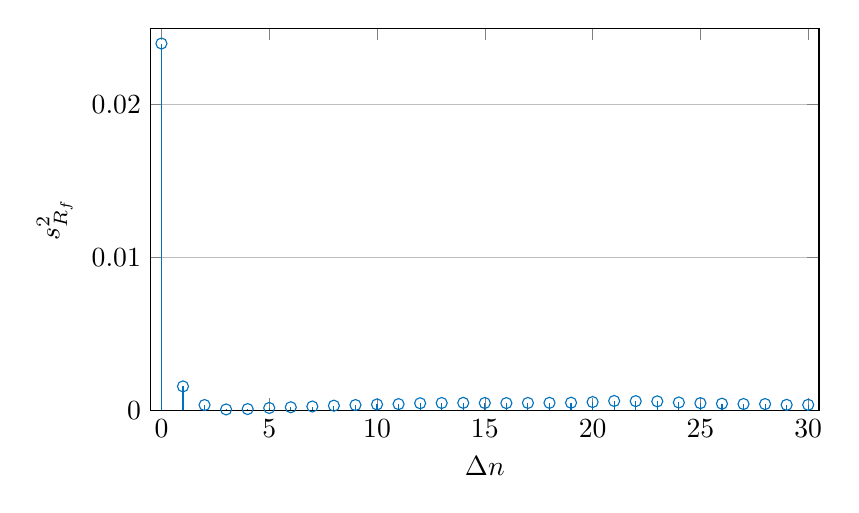
\begin{tikzpicture}

\begin{axis}[%
width=0.7\textwidth,
height=0.4\textwidth,
at={(0.758in,0.481in)},
scale only axis,
scaled y ticks = false,
y tick label style={/pgf/number format/fixed, /pgf/number format/precision=4},
xmin=-0.5,
xmax=30.5,
xlabel = $\Delta n$,
ymajorgrids,
ymin=0,
ymax=0.025,
ylabel = $s_{R_f}^2$,
axis background/.style={fill=white}
]
\addplot[ycomb,color=mycolor1,solid,mark=o,mark options={solid},forget plot] plot table[row sep=crcr] {%
0	0.0239994535570242\\
1	0.00155347561399147\\
2	0.000333132530399424\\
3	4.42952964310783e-05\\
4	6.91463617776512e-05\\
5	0.000140552123495002\\
6	0.00018743076774746\\
7	0.000236684877793891\\
8	0.000291324870818997\\
9	0.000331910825749033\\
10	0.000371904245897478\\
11	0.00039280175885968\\
12	0.000448157932287774\\
13	0.00046607349315818\\
14	0.000475171842259718\\
15	0.000466606546009396\\
16	0.000459354658352822\\
17	0.000469730606803343\\
18	0.000476346246957716\\
19	0.000483291253215299\\
20	0.00052789844826084\\
21	0.000599881231205234\\
22	0.000587411820871848\\
23	0.000573953897934685\\
24	0.000499460691984749\\
25	0.000456959069830855\\
26	0.000421847342166333\\
27	0.000400310575870904\\
28	0.000396373029801933\\
29	0.000345580578532402\\
30	0.000347170193328993\\
};
\end{axis}
\end{tikzpicture}%
\caption{Variance of autocorrelation with respect to $\Delta n$.}
\label{fig:var_freq}
\end{figure}

It can be seen from \autoref{fig:var_freq} that all the variences are quite low,this is a very good indicator that the autocorrelation is only dependet on $\Delta n$ and therfore the data is WSS.

\textbf{Spatial domain correlation}

Analogously to the frequency domain the process is repeated but for the spatial domain. The result of which can be seen on \autoref{fig:var_space}.

\begin{figure}[H]
\centering
% This file was created by matlab2tikz.
%
%The latest updates can be retrieved from
%  http://www.mathworks.com/matlabcentral/fileexchange/22022-matlab2tikz-matlab2tikz
%where you can also make suggestions and rate matlab2tikz.
%
\definecolor{mycolor1}{rgb}{0.00000,0.44700,0.74100}%
%
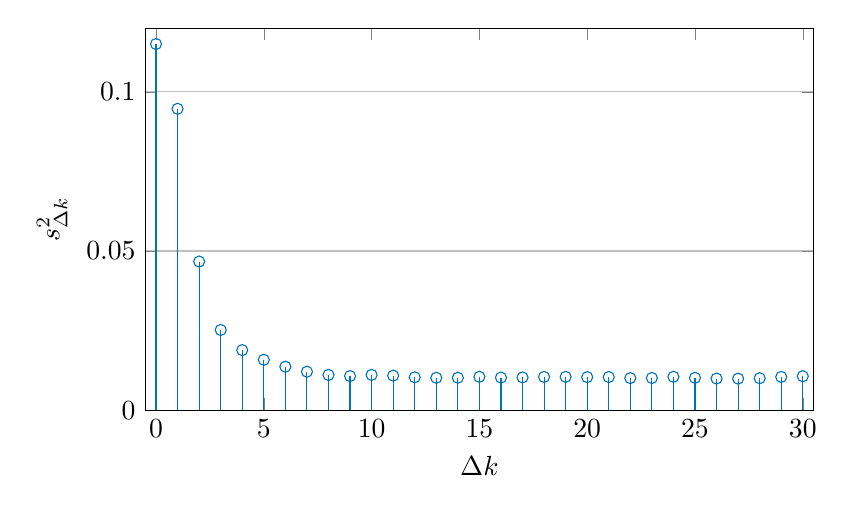
\begin{tikzpicture}

\begin{axis}[%
width=0.7\textwidth,
height=0.4\textwidth,
at={(0.758in,0.481in)},
scale only axis,
y tick label style={/pgf/number format/fixed},
xlabel = $\Delta k$,
xmin=-0.5,
xmax=30.5,
ymajorgrids,
ymin=0,
ymax=0.12,
ylabel = $s^2_{\Delta k}$,
axis background/.style={fill=white}
]
\addplot[ycomb,color=mycolor1,solid,mark=o,mark options={solid},forget plot] plot table[row sep=crcr] {%
0	0.115045606834225\\
1	0.0946784511696748\\
2	0.0466923552353349\\
3	0.0251857163185419\\
4	0.0188648457284451\\
5	0.0158108437878889\\
6	0.0136428154850336\\
7	0.0120691680816066\\
8	0.0110553269974913\\
9	0.0107016887908107\\
10	0.0110733653475015\\
11	0.0108419533225932\\
12	0.0103199849300731\\
13	0.0101549456533492\\
14	0.0101751416039882\\
15	0.010467137052642\\
16	0.0102326076635985\\
17	0.0102798250233889\\
18	0.0104377402107261\\
19	0.0104501815917102\\
20	0.010370718973987\\
21	0.0103919293729459\\
22	0.0100594042395687\\
23	0.0100951562316132\\
24	0.01047263290787\\
25	0.0101459206592842\\
26	0.00991026231424316\\
27	0.00989028804544289\\
28	0.0100207717725258\\
29	0.0104324957762442\\
30	0.0106517054365681\\
};
\end{axis}
\end{tikzpicture}%
\caption{Variance of autocorrelation with respect to $\Delta k$.}
\label{fig:var_space}
\end{figure}

It can be seen from \autoref{fig:var_space} that the variance is not nearly as small as for the frequency domain, this could be connected to the problem discovered from \autoref{fig:Not_norm_space} these two problems indicates that a dominant component has been received from the direction of the antenna. It is however assumed that the effect of this component is only big enough to be seen in the stationarity analysis and not in the result of the fading characteristic.
